\documentclass[../main.tex]{subfiles}
\graphicspath{{\subfix{../images/}}}
\begin{document}

\chapter{Introduction}%
\label{ch:introduction}

%% PDF 1 of Lecture Notes

\todo{Do we want to say a word about groups = symmetry and manifolds = calculus?}
\todo{Also, do we want to motivate these objects at all?}

\section{Lie Groups = Symmetry + Calculus}
  
\begin{defn}
  A \important{Lie Group} is a group in the category of manifolds.
\end{defn}

\begin{defn}
  A \important{Lie Group} is a group that is also a manifold%
  \footnote{and the operations should be smooth with respect to this structure.}.
\end{defn}

Given a Lie Group $G$, its tangent space at the identity is called a 
\important{Lie Algebra}, often written $\mathfrak{g}$.

\missingfigure{$S^1$ with the tangent line at the origin}

In this image, our group $G = \{ e^{i \theta} \mid \theta \in \R \}$,
and its lie algebra is $\mathfrak{g} = \{ i \theta \mid \theta \in \R \}$.

Lie algebras let us reduce problems about Lie groups to linear algebra.

\section{The Plan}
\todo{So this makes sense as part of a day 1 of lecture, but should we 
put this in a preface or something instead of right here?}

In this book, we'll cover

\begin{enumerate}
  \item \textbf{General Theorems} about Lie Groups and Lie Algebras \todo{Are we still planning to "skip many proofs?"}
  \item \textbf{Examples} -- These are the key to really \emph{understanding} Lie groups.
  \item \textbf{Applications} to 
    \begin{itemize}
      \item Geometry -- Felix Klein's idea \todo{cite the erlangen program, a historical account, or another book?}
        that a geometrical figure (a point, line, etc.) is "really" an action of a Lie group on a manifold.
      \item Quantum Physics -- The idea \todo{can we trace this to anyone like we can Klein?} a type of particle
        is "really" an action (or \emph{representation} in this context) of a Lie group on a Hilbert Space.
    \end{itemize}
\end{enumerate}

\section{A Review of Manifold Theory}

\begin{defn}
  An ($n$-dimensional) \important{Topological Manifold} is a topological space $M$ so that
  each point $x \in M$ has an open neighborhood $U_x$ homeomorphic to $\R^n$.

  We may also call $M$ an $n$-manifold.
\end{defn}

\todo{Add a thing in the preface that says %
``the reader familiar with Tu's intro to manifolds will recognize the influence on this section'' %
or something like that. I really did lift this almost verbatim.}

A fixed homeomorphism $U_x \to \R^n$ is called a \important{Chart}, and
we call two charts $\varphi : U \to \R^n$, $\psi : V \to \R^n$ 
\important{Compatible} if the two maps 
$\varphi \circ \psi^{-1} : \psi(U \cap V) \to \varphi(U \cap V)$ and 
$\psi \circ \varphi^{-1} : \varphi(U \cap V) \to \psi(U \cap V)$ are 
smooth (by which we mean $C^\infty$).

These two maps are called the \important{Transition Functions} between
the charts. 

\missingfigure{A figure indicating what it means for charts to be compatible}

\begin{defn}
  An \important{Atlas} on a topological manifold $M$ is a collection of 
  compatible charts whose domains cover $M$.

  An atlas is called \important{Maximal} if any chart $\varphi : X \to \R^n$
  not in the atlas is incompatible with some chart in the atlas.
\end{defn}

\begin{defn}
  An ($n$-dimensional) \important{Smooth Manifold} is a topological 
  $n$-manifold $M$ equipped with a maximal atlas. 

  Unless otherwise stated, by ``manifold'' we will always mean a smooth
  manifold. 
\end{defn}

\begin{ExerciseList}

\Exercise[label={ex:automatic-compatibility-of-charts}]
Let $\mathfrak{A}$ be an atlas on a topological manifold $M$. 
If $(U, \varphi)$ and $(V, \psi)$ are both compatible with every
chart in $\mathfrak{A}$, then they are compatible with each other too.

\Exercise[label={ex:atlases-extend-to-maximal-atlases}]
Every atlas $\mathfrak{A} = \{ (U_\alpha, \varphi_\alpha) \}$ on a 
topological manifold $M$ is contained in a (unique!) maximal atlas.
(Hint: consider all charts compatible with every chart in $\mathfrak{A}$,
then use the previous exercise to argue that this is still an atlas)

This exercise shows that we don't need to define a maximal atlas to put a 
smooth structure on a topological manifold. In practice, we almost always 
work with a much more manageable atlas with only finitely many charts.
  
\end{ExerciseList}

\bigskip

Where there are objects, there are arrows, and we should consider the 
maps between manifolds as well. 

\begin{defn}
  Let $M$ and $N$ be manifolds. A function $f : M \to N$ is called 
  \important{(Smooth) Map} if for every $x \in M$ there are charts
  $(U_x, \varphi)$ and $(V_{f(x)}, \psi)$ so that 
  $\psi \circ f \circ \phi^{-1}$ is smooth.
\end{defn}

\begin{ExerciseList}
  
\Exercise[label={ex:any-chart-works-for-smooth-map}]
Show that if the above definition works for \emph{some} charts
$(U_x, \varphi)$ and $(V_{f(x)}, \psi)$, it actually works for 
every pair of charts whose domains are neighborhoods of $x$ and $f(x)$.
(Hint: transition functions are smooth).

\end{ExerciseList}

\missingfigure{Indicate the definition of a smooth map with potatoes and arrows}

\begin{defn}
  The smooth manifolds and smooth maps together form the category $\mathsf{Diff}$.

  An isomorphism in this category%
  \footnote{that is, a pair of maps $f : M \to N$ and $g : N \to M$ so that 
  $f \circ g = \id_N$ and $g \circ f = \id_M$} is called a \important{Diffeomorphism}.

  We consider two diffeomorphic manifolds to be ``the same''.
\end{defn}

Let us define Lie Groups exactly one more time.

\begin{defn}
  A \important{Lie Group} is a manifold $G$ equipped with smooth maps 

  \begin{itemize}
      \item $\cdot : G \times G \to G$ 
      \item ${}^{-1} : G \to G$ 
  \end{itemize}

  and a point $1 \in G$ so that $(G,1,\cdot, {}^{-1})$ is a group.
\end{defn}

The attentive reader will notice the sleight of hand. What does it mean
to have a smooth map from $G \times G \to G$? We know that $G$ is a manifold
by assumption, but why should $G \times G$ be one!? 

\begin{defn}
  Given an $m$-manifold $M$ and an $n$-manifold $N$ 
  (with atlases $\mathfrak{A}$ and $\mathfrak{B}$, respectively), the 
  product topological space $M \times N$ becomes an $(m+n)$-manifold by
  considering the atlas

  \[
    \big \{ 
      (U \times V, \varphi \times \psi) 
    \mid 
      (U, \varphi) \in \mathfrak{A}, (V, \psi) \in \mathfrak{B} 
    \big \}
  \]

  (which we can extend to a maximal atlas by exercise 
  \ref{ex:atlases-extend-to-maximal-atlases})

\end{defn}

\todo{Do we want to prove that this really is a manifold? Or leave it as an exercise? Or not mention it at all?}

\begin{ExerciseList}
  \Exercise[label={ex:categorical-product-of-manifolds}]
  Prove that this construction really is a product in the categorical sense. 
  That is, show 

  \begin{enumerate}
    \item The topological projection maps $\pi_1 : M \times N \to M$ and 
      $\pi_2 : M \times N \to N$ are smooth
    \item For any manifold $X$ and for any maps $f : X \to M$ and $g : X \to N$,
      there is a unique map $f \times g : X \to M \times N$ making the following
      diagram commute:
  \end{enumerate}

  \missingfigure{You know the one}
\end{ExerciseList}

\section{Examples of Lie Groups}

\todo{You said (out loud) a lot of words about each of these examples. 
I can try to imitate your voice, or you can write some words here. 
Let me know what you prefer.}
  
\subsection{$(\R^n, +)$}

More generally, any real or complex vector space $V$ becomes a Lie group 
under vector addition.

\subsection{$\mathsf{GL}(n,\R)$}

\begin{defn}
  The ($n \times n$, real) \important{General Linear Group} 

  \[ \mathsf{GL}(n,\R) = \big \{ \text{invertible $n \times n$ matrices with entries in $\R$} \big \} \]

  is a Lie group with matrix multiplication as its operation.
\end{defn}

This is clearly a group, but why is it a manifold, and why are multiplying
and inverting matrices smooth operations?

The key observation is that $\mathsf{GL}(n,\R)$ is an open subset of 
$\mathcal{M}(n,\R)$ (the space of all matrices), which is an $n^2$-dimensional
vector space (and thus a manifold).

This is because $\text{det} : \mathcal{M}(n,\R) \to \R$ is a polynomial in
the entires of the matrix, thus it's continuous (smooth, even!) and 
$\mathsf{GL}(n,\R) = \text{det}^{-1} \{ x \in \R \mid x \neq 0 \}$ is an 
open subset of $\mathcal{M}(n,\R)$.

So to know that $\mathsf{GL}(n,\R)$ is a manifold, it's enough to show

\begin{thm}
  An open subset of an $n$-manifold is an $n$-manifold
\end{thm}

\begin{proof}
  I'm feeling lazy right now.

  \missingfigure{The visual from the notes showing what's happening}
\end{proof}

So $\mathsf{GL}(n,\R)$ is a manifold. Why is it a Lie group?

Notice multiplication

\[
  (A,B) \mapsto (AB)_{i,j} = \sum_k A_{ik} B_{kj}
\]

and inversion

\[
  A \mapsto A^{-1}_{ij} = \frac{(-1)^{i+j} \text{minor}_{ji}}{\text{det}(A)}
\]

are both polynomial maps. In particular, they're smooth.

\todo{I should probably double check that the inversion formula is exactly right.
It's definitly \emph{something} like this\ldots}

\todo{Also, we should probably put in a few more words about what minors are, etc?
Either that, or call this an exercise, and say "consider the minors", etc as a hint?}

\bigskip

It will come as no surprise that we can use $\C$ instead of $\R$ above, and
everything goes through unchanged.

\begin{defn}
  The ($n \times n$, complex) \important{General Linear Group} is

  \[
    \mathsf{GL}(n,\C) = \big \{ \text{invertible $n \times n$ matrices with entries in $\C$} \big \}.
  \]

  This is a Lie group with matrix multiplication and inversion.
\end{defn}

Again, this is a manifold because it is an open subset of the $2n^2$-dimensional
(real) vector space $\mathcal{M}(n,\C)$ of $n \times n$ complex matrices and
the group operations are polynomials (thus smooth).

\subsection{Closed Subgroups}

We can also get new Lie groups from old.

\begin{thm}
  A closed subgroup%
  \footnote{That is, if $H$ is a subgroup of $G$ which is topologically closed} 
  of a Lie group $G$ is itself a Lie group.
\end{thm}

\begin{proof}
  $H$ is a submanifold of $G$, and the group operations restrict to smooth
  maps on $H$. For a formal proof (which would take us into more manifold 
  theory than we would like), see F. Warner's 
  \emph{Foundations of Differentiable Manifolds and Lie Groups}, p. 110
  (I stole this reference from Tu's book).
  \todo{This is the first of many theorems which we didn't \emph{really} prove
  in lecture. I personally think we should 
  keep the philosophy of ``don't prove everything'', and just provide a 
  reference where the proof normally goes (as I did here). If we're doing this, 
  we should mention it in the preface}
\end{proof}

With this theorem in hand, we'll get a whole slew of new examples of Lie groups
by considering the closed subgroups of $\mathsf{GL}(n,\C)$!

%% PDF 2 of Lecture Notes

\section{Matrix Lie Groups}

\todo{In the handwriten notes, you mentioned homomorphisms here. 
I think it flows better to move straight into matrix lie groups, 
and mention homs and the category of lie groups after. Let me know
if you have a reason for putting the order back how you had it}

\begin{defn}
A \important{Matrix Lie Group} is a closed subgroup of $\mathsf{GL}(n,\C)$. 
\end{defn}

\todo{This is a kind of subtle formatting thing that may not matter.
I'm currently doing these as subsections, but they're all quite short\ldots
Do you think it makes more sense to make this an enumerate instead?}

\subsection{$\mathsf{GL}(n,\R)$}

We've already met $\mathsf{GL}(n,\R)$, which certainly deserves to be called 
a ``matrix Lie group''. Why is this formally the case, though?

Well this is obviously a subgroup of $\mathsf{GL}(n,\C)$, so we just need to 
show that it's \emph{closed}. So let's fix a sequence of matrices 
$A_n$ converging to $A$ with each $A_n \in \mathsf{GL}(n,\R)$. We want to
show $A$ is in $\mathsf{GL}(n,\R)$ too.

But $A_n \to A$ if and only if each entry $(A_n)_{i,j} \to A_{i,j}$! 
So we have $n^2$ many convergent real sequences, and each sequence must
have its limit in $\mathbb{R}$. But that means each entry $A_{i,j}$ is 
real, and so $A \in \mathsf{GL}(n,\R)$.

\subsection{$\mathsf{SL}(n,\C)$}

\begin{defn}
  The \important{(Complex) Special Linear Group} is the set of $n \times n$ complex
  matrices of determinant $1$:

  \[
    \mathsf{SL}(n,\C) = \{ A \in \mathsf{GL}(n,\C) \mid \text{det}(A) = 1 \}
  \]
\end{defn}

\begin{ExerciseList}
  \Exercise[label={ex:SLn-subgroup}] Prove $\mathsf{SL}(n,\C)$ is a subgroup of $\mathsf{GL}(n,\C)$
  (Hint: $\text{det}(AB) = \text{det}(A) \text{det}(B)$)

  \Exercise[label={ex:SLn-closed}] Prove $\mathsf{SL}(n,\C)$ is closed in $\mathsf{GL}(n,\C)$
  (Hint: $\text{det}$ is a continuous function, and $\{1\}$ is closed in $\C$)
\end{ExerciseList}

\subsection{$\mathsf{SL}(n,\R)$}

\begin{defn}
  The \important{(Real) Special Linear Group} is the set of $n \times n$ real
  matrices of determinant $1$:

  \[
    \mathsf{SL}(n,\R) = \{ A \in \mathsf{GL}(n,\R) \mid \text{det}(A) = 1 \}
  \]
\end{defn}

Notice $\mathsf{SL}(n,\R) = \mathsf{GL}(n,\R) \cap \mathsf{SL}(n,\C)$ is the 
intersection of closed subgroups of $\mathsf{GL}(n,\C)$, and thus is itself
a closed subgroup\footnote{recall that separately the intersection of closed sets is closed, 
and the intersection of subgroups is a subgroup}.
  
\subsection{$\mathsf{U}(n)$}

\begin{defn}
  The \important{Unitary Group} is the set of $n \times n$ unitary matrices

  \[
    \mathsf{U}(n) = \{ A \in \mathsf{GL}(n,\C) \mid A A^* = 1 \}
  \]

  where, as usual $A^*$ is the \important{Adjoint} 
  (or \important{Conjugate Transpose}) $(A^*)_{i,j} = \overline{A_{j,i}}$.
\end{defn}

\begin{ExerciseList}
  \Exercise[label={ex:Un-subgroup}] Prove $\mathsf{U}(n)$ is a subgroup of $\mathsf{GL}(n,\C)$.

  \Exercise[label={ex:Un-closed}] Prove $A \mapsto A^*$ is continuous. Use this to 
  conclude that $A \mapsto A A^*$ is continuous, and thus that $\mathsf{U}(n)$ is closed.
\end{ExerciseList}

\todo{This is the only matrix group that gets an extra lemma. 
I think you gave some exposition about how important a group this is,
and it might be worth including some exposition here as well?}

\begin{lemma}
  For any $g \in \mathsf{GL}(n,\C)$, the following are equivalent:

  \begin{enumerate}
    \item $g g^* = 1$
    \item $g^* g = 1$
    \item $g$ preserves inner products. That is, 
      $\langle gv, gw \rangle = \langle v, w \rangle$
      for every $v$ and $w$ in $\C^n$. Here we use the
      inner product $\langle v, w \rangle = \sum \overline{v_i} w$.
    \item $g$ preserves lengths. That is,
      $\norm{gv} = \norm{v}$ for every $v \in \C^n$. Here
      $\norm{v} = \sqrt{\langle v, v \rangle}$.
  \end{enumerate}
\end{lemma}

\begin{proof}
  $1 \iff 2$ is easy, since any left inverse is a right inverse and vice versa.

  $2 \iff 3$ follows from $\langle gv, gw \rangle = \langle v, g^* g w \rangle$

  $3 \implies 4$ is clear, since $\norm{\cdot}$ is defined in terms of $\langle \cdot, \cdot \rangle$.

  $4 \implies 3$ requires a little trick called ``polarization'' which is good to have
  in your back pocket. We can actually recover $\langle \cdot, \cdot \rangle$ 
  from the norm with the following formula:

  \[ \langle v, w \rangle = \frac{1}{4} \left ( \norm{v+w}^2 - \norm{v-w}^2 \right ) \]

  Since we can define $\langle \cdot , \cdot \rangle$ from $\norm{\cdot}$
  and we know $g$ preserves $\norm{\cdot}$, we see $g$ must \emph{also} preserve
  the inner product.
\end{proof}

This lets us give a more conceptual justification why $\mathsf{U}(n)$ is a
subgroup of $\mathsf{GL}(n,\C)$. In general, if you have a group that acts
on a structure, then anytime you look at those group elements which preserve
$\sim$ bonus structure $\sim$, you'll actually be looking at a subgroup.

In this case, $\mathsf{GL}(n,\C)$ acts on $\C^n$ (by matrix-vector multiplication),
and $\mathsf{U}(n)$ are exactly those elements preserving the 
$\sim$ bonus structure $\sim$ called ``length''.

\subsection{$\mathsf{O}(n)$}

\begin{defn}
  The \important{Orthogonal Group} is the set of $n \times n$ orthogonal matrices

  \[ 
    \mathsf{O}(n) = \{ A \in \mathsf{GL}(n,\R) \mid AA^* = 1 \}
  \]

  Note since $A$ is real, we have $A^* = A^T$.
\end{defn}

This is a closed subgroup since it is the intersection of two closed subgroups
(do you see which ones?)

\subsection{$\mathsf{SU}(n)$}

\begin{defn}
  The \important{Special Unitary Group} is the set of $n \times n$ matrices

  \[
    \mathsf{SU}(n) = \{ A \in \mathsf{GL}(n,\C) \mid A A^* = 1 \text{ and } \text{det}(A) = 1 \}
  \]
\end{defn}

This is a closed subgroup since it is the intersection of two closed subgroups
(do you see which ones?)

\subsection{$\mathsf{SO}(n)$}

\begin{defn}
  The \important{Special Orthogonal Group} is the set of $n \times n$ matrices
  \[
    \mathsf{SO}(n) = \{ A \in \mathsf{GL}(n,\R) \mid A A^* = 1 \text{ and } \text{det}(A) = 1 \}
  \]
\end{defn}

This is a closed subgroup since it is the intersection of two closed subgroups
(do you see which ones?)

\todo{You say in the notes that $SO(3)$ is the group of rotations in $\R^3$. 
Should we say more about that?}

\todo{Do we want to make these last $3$ a bit more distinct? Or otherwise add
some exposition for each? I made the presentation as an intersection implicit
exercises in each case to try and make the reader pay marginally more attention
amid the veritable deluge of definitions. Especially since we're going to be 
showing a big commutative diagram of inclusions on the next page that gives the
answer away.}

\section{Lie Group Homomorphisms}

Since Lie groups have the structure of both a group and a manifold, 
we want our homomorphisms to preserve both of these structures. With that
in mind, we define

\begin{defn}
  A \important{Lie Group Homomorphism} $f$ between Lie groups $G$ and $H$ 
  is a group homomorphism which is also a smooth map.

  Unsurprisingly, Lie Groups and their homomorphisms assemble into a category
  $\mathsf{LieGrp}$.
\end{defn}

One important example of a Lie group homomorphism is the inclusion of a 
closed subgroup $H \subseteq G$ into $G$. \todo{Say a word about why this is smooth?}

In particular, if $H$ is a matrix Lie group, then for some $n$ 
we have a $1$-to-$1$ Lie group homomorphism 
$\iota : H \hookrightarrow \mathsf{GL}(n,\C)$.

In fact, we can put together all of the groups we've seen so far into one 
diagram that shows the relations between them:

\[\begin{tikzcd}
	& {\mathsf{GL}(n,\mathbb{R})} &&& {GL(n,\mathbb{C})} \\
	&& {\mathsf{O}(n)} &&& {\mathsf{U}(n)} \\
	{\mathsf{SL}(n,\mathbb{R})} &&& {\mathsf{SL}(n,\mathbb{C})} \\
	& {\mathsf{SO}(n)} &&& {\mathsf{SU}(n)}
	\arrow[hook, from=4-2, to=3-1]
	\arrow[hook, from=3-1, to=1-2]
	\arrow[hook, from=4-2, to=2-3]
	\arrow[hook, from=2-3, to=1-2]
	\arrow[hook, from=4-5, to=2-6]
	\arrow[hook, from=4-5, to=3-4]
	\arrow[hook, from=3-4, to=1-5]
	\arrow[hook, from=2-6, to=1-5]
	\arrow[hook, from=1-2, to=1-5]
	\arrow[hook, from=3-1, to=3-4]
	\arrow[hook, from=4-2, to=4-5]
	\arrow[hook, from=2-3, to=2-6]
\end{tikzcd}\]

\section{Concrete Examples: Low Dimensions}

Let's look at the above diagram in the case $n = 1$

\todo{Should we say something more about each of these?}

\begin{itemize}
    \item $\mathsf{GL}(1,\C) \cong \C^\times                   \cong (\C \setminus \{ 0 \}, \cdot)$
    \item $\mathsf{GL}(1,\R) \cong \R^\times                   \cong (\R \setminus \{ 0 \}, \cdot)$
    \item $\mathsf{U}(1)     \cong \{ z \in \C \mid |z| = 1 \} \cong S^1$ is the \important{Circle Group}
    \item $\mathsf{O}(1)     \cong \{ x \in \R \mid |x| = 1 \} \cong \mathbb{Z} / 2 \cong S^0$
\end{itemize}

\todo{In the notes these are all the examples given, because things trivialize a little in this dimension.
Do we want to say something about that? There's examples in dimension $2$ coming up, so maybe we don't need to?}

\todo{This note also kind of comes out of nowhere. We should maybe say something to make it feel a bit more
cohesive with the surrounding text.}

Note:

\begin{align*}
  \mathsf{GL}(1,\C) 
  &\cong \mathbb{C}^\times \\
  &\cong \{ r e^{i \theta} \mid r, \theta \in \R \} \\
  &\cong \mathbb{R} \times S^1
\end{align*}

\begin{align*}
  \mathsf{GL}(1,\R)
  &\cong \mathbb{R}^\times \\
  &\cong \{ e^{r} \eps \mid r \in \R, \eps = \pm 1 \} \\
  &\cong \mathbb{R} \times S^0
\end{align*}

\missingfigure{$\mathsf{GL}(1,\C)$ as a punctured disk vs as a cylinder. $\mathsf{GL}(1,\R)$ is highlighted inside it.}

%% PDF 3 of lecture notes

Now let's look in dimension $2$!

$\mathsf{GL}(2,\R)$ are the linear transformations of the plane. For instance,
these are all transformations in $\mathsf{GL}(2,\R)$.

\todo{figure out how to center these nicely and add a $\mapsto$ in between these}

\begin{align*}
  (1) && 
\begin{pmatrix}
  0 & -1 \\ 1 & 0
\end{pmatrix}
  &&&
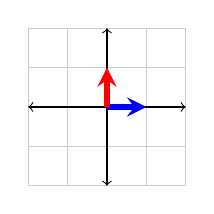
\begin{tikzpicture}[scale=0.5]
  \draw[thin,gray!40] (-2,-2) grid (2,2);
  \draw[<->] (-2,0)--(2,0);
  \draw[<->] (0,-2)--(0,2);
  \draw[line width=2pt,blue,-stealth](0,0)--(1,0);
  \draw[line width=2pt,red,-stealth](0,0)--(0,1);
\end{tikzpicture}
  &&&
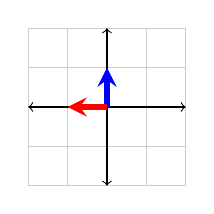
\begin{tikzpicture}[scale=0.5]
  \draw[thin,gray!40] (-2,-2) grid (2,2);
  \draw[<->] (-2,0)--(2,0);
  \draw[<->] (0,-2)--(0,2);
  \draw[line width=2pt,blue,-stealth](0,0)--(0,1);
  \draw[line width=2pt,red,-stealth](0,0)--(-1,0);
\end{tikzpicture} \\
  (2) && 
\begin{pmatrix}
  0 & 1 \\ 1 & 0
\end{pmatrix}
  &&&
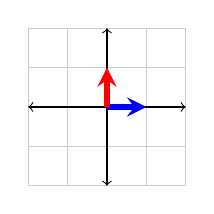
\begin{tikzpicture}[scale=0.5]
  \draw[thin,gray!40] (-2,-2) grid (2,2);
  \draw[<->] (-2,0)--(2,0);
  \draw[<->] (0,-2)--(0,2);
  \draw[line width=2pt,blue,-stealth](0,0)--(1,0);
  \draw[line width=2pt,red,-stealth](0,0)--(0,1);
\end{tikzpicture}
  &&&
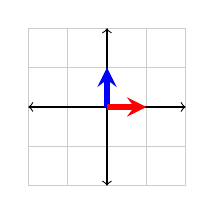
\begin{tikzpicture}[scale=0.5]
  \draw[thin,gray!40] (-2,-2) grid (2,2);
  \draw[<->] (-2,0)--(2,0);
  \draw[<->] (0,-2)--(0,2);
  \draw[line width=2pt,blue,-stealth](0,0)--(0,1);
  \draw[line width=2pt,red,-stealth](0,0)--(1,0);
\end{tikzpicture} \\
  (3) && 
\begin{pmatrix}
  1 & 1 \\ 0 & 1
\end{pmatrix}
  &&&
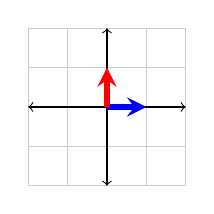
\begin{tikzpicture}[scale=0.5]
  \draw[thin,gray!40] (-2,-2) grid (2,2);
  \draw[<->] (-2,0)--(2,0);
  \draw[<->] (0,-2)--(0,2);
  \draw[line width=2pt,blue,-stealth](0,0)--(1,0);
  \draw[line width=2pt,red,-stealth](0,0)--(0,1);
\end{tikzpicture}
  &&&
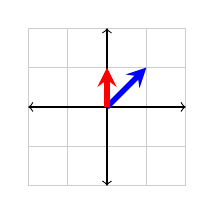
\begin{tikzpicture}[scale=0.5]
  \draw[thin,gray!40] (-2,-2) grid (2,2);
  \draw[<->] (-2,0)--(2,0);
  \draw[<->] (0,-2)--(0,2);
  \draw[line width=2pt,blue,-stealth](0,0)--(1,1);
  \draw[line width=2pt,red,-stealth](0,0)--(0,1);
\end{tikzpicture} \\
  (4) &&
\begin{pmatrix}
  2 & 0 \\ 0 & 1
\end{pmatrix}
  &&&
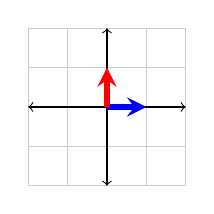
\begin{tikzpicture}[scale=0.5]
  \draw[thin,gray!40] (-2,-2) grid (2,2);
  \draw[<->] (-2,0)--(2,0);
  \draw[<->] (0,-2)--(0,2);
  \draw[line width=2pt,blue,-stealth](0,0)--(1,0);
  \draw[line width=2pt,red,-stealth](0,0)--(0,1);
\end{tikzpicture}
  &&&
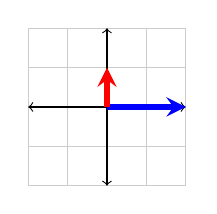
\begin{tikzpicture}[scale=0.5]
  \draw[thin,gray!40] (-2,-2) grid (2,2);
  \draw[<->] (-2,0)--(2,0);
  \draw[<->] (0,-2)--(0,2);
  \draw[line width=2pt,blue,-stealth](0,0)--(2,0);
  \draw[line width=2pt,red,-stealth](0,0)--(0,1);
\end{tikzpicture} 
\end{align*}

Now $\mathsf{O}(2)$ is the set of all linear transformations
that preserve inner products (thus angles and lengths), and
$\mathsf{SL}(2,\R)$ are those transformations preserving oriented areas.

So examples $1$ and $2$ are in $\mathsf{O}(2)$, and examples $1$ and $3$ are 
in $\mathsf{SL}(2,\R)$ (do you see why?). Notice that even though areas are 
preserved in example $2$, the \emph{orientation} of the area changes. That is,
before the transformation is applied, moving from the blue to the red vector
is a clockwise motion, while after the transformation, moving from blue to red
is a counterclockwise motion.

\missingfigure{The same pictures as in $(2)$, but with big curvey arrows from blue to red}

Lastly $\mathsf{SO}(2) = \mathsf{O}(2) \cap \mathsf{SL}(2,\R)$ consists of exactly
the rotations. That is,

\[ 
  \mathsf{SO}(2) = 
  \left \{ 
    \begin{pmatrix} 
      \cos \theta & - \sin \theta \\ \sin \theta & \cos \theta 
    \end{pmatrix}
  \mid
    \theta \in \R
  \right \}
\]

\begin{ExerciseList}
  \Exercise like\ldots $5$ or $6$ matrices, and ask which is in each major Lie group

  \Exercise like\ldots $5$ or $6$ pictures of $2D$ transformations like earlier,
  ask which is in each major Lie group.
\end{ExerciseList}

\subsection{Visualizing Low Dimensional Lie Groups}

So, as Lie groups, 

\todo{idk why this is aligning so uglily\ldots}
\begin{align*}
  \mathsf{SO}(2) &\cong S^1           &= \R \big / 2\pi \Z  \\
                 &\cong \mathsf{U}(1) &= \{ z \in \C \mid |z| = 1 \}
\end{align*}

and $\mathsf{SO}(2)$ is exactly a circle.

What about $\mathsf{O}(2)$?

\begin{lemma}
  If $g \in \Un$, then $\abs{\text{det}(g)} = 1$.
\end{lemma}

\begin{proof}
  We know that 
  \[ 
    \text{det}(g g^*) 
    = \text{det}(g) \text{det}(g^*) 
    = \text{det}(g) \overline{\text{det}(g)}.
  \]

  so if $gg^* = 1$ we see $\abs{\text{det}(g)}^2 = 1$.
\end{proof}

\begin{cor}
  If $g \in \On$, then $\text{det}(g) = \pm 1$.
\end{cor}

So for $g \in \On$, either $g \in \SOn$ or $rg \in \SOn$ where
$r = \begin{pmatrix} -1  & 0 & \cdots & 0 \\ 0 & 1 & \cdots & 0 \\ \vdots & \vdots & \ddots & \vdots \\ 0 & 0 & \cdots & 1 \end{pmatrix}$
is a reflection. 

So as a \emph{manifold}, $\On \cong \SOn \sqcup \SOn$. In particular,
$\mathsf{O}(2)$ looks like two disjoint circles.

\todo{screw around with mdframed settings and make this look prettier.}

\begin{mdframed}
  Question: Do we have $\mathsf{O}(2) \cong \Z / 2 \times \mathsf{SO}(2)$ as Lie groups?

  What about $\mathsf{O}(3) \cong \Z / 2 \times \mathsf{SO}(3)$?
\end{mdframed}

\todo{In the notes we made a big deal out of these questions. We should
mention them as motivating problems if we're planning to come back to it,
and talk about what tools we need to develop to answer them}

To better understand $\mathsf{SL}(2, \R)$, we cleverly write our matrix as

\[
  g = \begin{pmatrix} x+z & w-y \\ w+y & x-z \end{pmatrix}
\]

with $w,x,y,z \in \R$.

Then $\text{det}(g) = x^2 + y^2 - z^2 - w^2$, and as a manifold

\[
  \mathsf{SL}(2,\R) \cong \{ (x,y,z,w) \in \R^4 \mid x^2 + y^2 = z^2 + w^2 + 1 \}.
\]

The slice $w=0$ is a hyperboloid with one sheet:

\missingfigure{a hyperboloid with one sheet}

This is diffeomorphic to $\R \times S^1$.

So $\mathsf{SL}(2,\R)$ is diffeomorphic to $\R^2 \times S^1$, since for each
choice of $(z,w) \in \R^2$ we get a circle $x^2 + y^2 = z^2 + w^2 + 1$. 

In fact, the circle $z=w=0$ is exactly $\mathsf{SO}(2) \subseteq \mathsf{SL}(2, \R)$!

\[
\left \{
  \begin{pmatrix}
    x+z & w-y \\ w+y & x-z
  \end{pmatrix}
\middle |
  \begin{aligned}
    x^2 + y^2 &= z^2 + w^2 + 1 \\ z&=w=0
  \end{aligned}
\right \}
=
\left \{ 
  \begin{pmatrix}
    x & -y \\ y & x
  \end{pmatrix}
\middle |
  x^2 + y^2 = 1
\right \}
=
\left \{ 
  \begin{pmatrix}
    \cos \theta & - \sin \theta \\ \sin \theta & \cos \theta
  \end{pmatrix}
\middle |
  \theta \in \R
\right \}
\]

So we can picture a slice of $\mathsf{SL}(2, \R)$ like this

\missingfigure{A hyperboloid with a section corresponding to $\mathsf{SO}(2)$}

\warning -- $\mathsf{SL}(2, \R)$ is diffeomorphic to $\mathsf{SO}(2) \times \R^2$,
but they are \emph{not} isomorphic as Lie groups! Indeed $\mathsf{SL}(2, \R)$ is
nonabelian, while $\mathsf{SO}(2) \times \R^2$ \emph{is} abelian! (do you see why?)

There is actually a deep theorem hiding inside this observation:

\begin{thm}
  ANy connected Lie group $G$ is diffeomorphic to $K \times \R^n$ where
  $K \subseteq G$ is a \important{Maximal Compact Subgroup} of $G$. That is,
  a compact subgroup not contained in a bigger compact subgroup.

  All maximal compact subgroups are conjugate, thus isomorphic as Lie groups.
\end{thm}

As another example of this theorem, recall $\mathsf{GL}(1,\C) \cong \mathsf{U}(1) \times \R$:

\missingfigure{A cylinder, with a section corresponding to $\mathsf{U}(1)$}

In fact:

\begin{thm}
  \begin{itemize}
    \item $\Un$ is a maximal compact subgroup of $\GLnC$   
    \item $\SUn$ is a maximal compact subgroup of $\SLnC$
    \item $\On$ is a maximal compact subgroup of $\GLnR$
    \item $\SOn$ is a maximal compact subgroup of $\SLnR$
  \end{itemize}
\end{thm}

If we color the compact Lie groups in red, as well as the inclusions
of maximal compact subgroups into larger Lie groups, we can summarize this
information as follows:

\[\begin{tikzcd}
	& {\mathsf{GL}(n,\mathbb{R})} &&& {GL(n,\mathbb{C})} \\
  && {\color{red}{\mathsf{O}(n)}} &&& {\color{red}{\mathsf{U}(n)}} \\
	{\mathsf{SL}(n,\mathbb{R})} &&& {\mathsf{SL}(n,\mathbb{C})} \\
  & {\color{red}{\mathsf{SO}(n)}} &&& {\color{red}{\mathsf{SU}(n)}}
	\arrow[hook, from=4-2, to=3-1, color=red]
	\arrow[hook, from=3-1, to=1-2]
	\arrow[hook, from=4-2, to=2-3]
	\arrow[hook, from=2-3, to=1-2, color=red]
	\arrow[hook, from=4-5, to=2-6]
	\arrow[hook, from=4-5, to=3-4, color=red]
	\arrow[hook, from=3-4, to=1-5]
	\arrow[hook, from=2-6, to=1-5, color=red]
	\arrow[hook, from=1-2, to=1-5]
	\arrow[hook, from=3-1, to=3-4]
	\arrow[hook, from=4-2, to=4-5]
	\arrow[hook, from=2-3, to=2-6]
\end{tikzcd}\]

\todo{This next bit feels somewhat jarring coming from what we've been
talking about. Maybe we can say a bit more to ease into it?}

In fact, \emph{any} inner product $(\cdot, \cdot)$ on $\C^n$ picks out a 
maximal compact subgroup of $\GLnC$, namely 
$K = \{ g \in \GLnC \mid (gv,gw) = (v,w) \}$.
Of course, these are all isomorphic to $U(n)$ (as the theorem above claims).

Similarly, any inner product on $\R^n$ picks out a maximal compact subgroup of
$\GLnR$.

\section{Quaternions and Visualizing $\mathsf{SU}(2)$}

%% PDF 4 of lecture notes

\todo{This is obviously long enough to warrent its own section, 
particularly since we're introducing quaternions here. But it seems a
bit strange to go back to visualizing after we took a digression into
maximal compact subgroups\ldots Maybe we say a word \emph{before} the digression
about how we'll talk about $\mathsf{SU}(2)$ soon, which justifies our coming 
back to it now?}




\end{document}

